\documentclass[12pt,svgnames,table]{beamer}
\usetheme{progressbar}

\usepackage[utf8x,utf8]{inputenc}
\usepackage{tikz}
\usetikzlibrary{decorations.pathmorphing}
\usepackage{xcolor}
\usepackage{amsmath,amsfonts,amsthm, amssymb}
\usepackage[babel=true]{csquotes}
\usepackage{etoolbox}
\usepackage{dsfont}
\usepackage{chngpage}



\usepackage{graphics} %% TOUT NEW!!
\usepackage{pgfplots} %% TOUT NEW!!  virer si pbm

%\usepackage{amsfonts}
%\usepackage[cmex10]{amsmath}
%\usepackage{multirow}
%\usepackage{amssymb}
%\usepackage{hyperref}
%\usepackage{graphicx}
%\usepackage{amssymb}
%\usepackage{amsmath}
%\usepackage{amsthm}
%\usepackage{dsfont}
%\usepackage{caption}
%\usepackage{graphicx}
%\usepackage{pgfplots}
%\usepackage{tikz}

\usetikzlibrary{shapes,snakes}

%\usepackage{txfonts}
%\usepackage{MnSymbol} % symbol independent
\newcommand{\paren}[1]{\left( \left. #1 \right. \right)} 
\newcommand{\croch}[1]{\left[ \left. #1 \right. \right]} 
\newcommand{\set}[1]{\left\{ \left. #1 \right. \right\}}
\newcommand{\sachant}{\, \right| \left. \,}
\newcommand{\nico}[1]{ }
\newcommand{\nicoo}[1]{#1}
% Modifiez ou necessaire:
% titre de these/topo

\title{
\vspace{0.7cm}\\
PIR : Mixed-Initiative Mission}

\normalsize
\author{\vspace{2cm} \textbf{Thomas Vagneron}}
% X=annee de these, Y=departement
\def\aboutauthor{\vspace{0.2cm}\hspace{-2.55cm} 
%under \textbf{D.Dubois}, \textbf{J-L.Farges} and \textbf{F.Teichteil-K\"onigsbuch} supervision\\
%\vspace{0.1cm}\hspace{-2.4cm} \textbf{doctoral school:} EDSYS \hspace{0.2cm} \textbf{institution:} ISAE--SUPAERO\\
%\vspace{0.1cm}\hspace{-3.2cm}\textbf{laboratory:} ONERA--The French Aerospace Lab\\ 
%\vspace{0.5cm} \hspace{0.2cm} 
\includegraphics[scale=0.45]{logo2015} \hspace{4.8cm}
%\begin{tikzpicture}
%\node[opacity=1] at (0,0) {\includegraphics[scale=0.35]{Logo_EDSYS2}};
%\end{tikzpicture}
}

% directeur de these
%\def\directeur{Toulouse}
% encadrant; s'il n'y a pas d'encadrant, veuillez commenter la ligne ci-dessous
%\def\encadrant{DCSD}


% Debut du documment
\begin{document}

% la premiere page
{
\usebackgroundtemplate{
\includegraphics[width=\paperwidth,height=\paperheight]{image_fond}} 
\begin{frame}[plain]
	\titlepage
\end{frame}
}
\section[summary]{summary}
\begin{frame}
\frametitle{Summary}
\begin{itemize}
 \item Context
 \item Theory
 \item Experiment
 \item Conclusion
 \end{itemize}
\end{frame}
\section[context]{Context and Goal}
\begin{frame}
\frametitle{\insertsection} 
\framesubtitle{\footnotesize Human-machine systems}
\begin{block}{Increasing use of automated systems}
aircrafts, cars or even games player (A fresh example is AlphaGo which is a Go playing machine).\\
\end{block}
\visible<2->{
\begin{itemize}
\item \textbf{Increasingly autonomous robots:}\\ 
technical advances in AI, machine learning. 
%deterministic behavior conditional to feedbacks/observations (policies)
\visible<3->{
\item \textbf{Human operator still vital:}\\
%more powerful for a vast majority of tasks 
- judiciary responsible \\
- able of creativity or improvisation.
%(robot can apply optimal decisions for known systems)
}
\end{itemize}
}
\visible<4->{
\begin{alertblock}{}
Human factors involved in $80\%$ of AAVs accidents! \cite{Williams04asummary}
\end{alertblock}
}
\end{frame}

\begin{frame}
\frametitle{\insertsection} 
\framesubtitle{\footnotesize Human operator weaknesses}
\textbf{Potential effects of a mission on human operators:}
\begin{itemize}
\item stress (danger, pressure)
\item workload (multi-task, hard tasks)
\item fatigue, boredom (long mission)
\end{itemize}
\visible<2->{
\textbf{Consequences:}
\begin{itemize}
\item mental confusion
\item attentional tunneling
\item mind wandering
\item lower vigilance
\item ...
\end{itemize}
}
\visible<2->{
\begin{alertblock}{}
\center increase in accident risk resulting in mission fails 
\end{alertblock}
}
\end{frame}
\begin{frame}
\frametitle{\insertsection}
\framesubtitle{\footnotesize use of human state feedbacks!}
\begin{block}{Human operators equipped with sensors}
\center data from the human operator state can\\  
\textbf{refine supervision of human-robot team}
\end{block}
\visible<2->{
\begin{itemize}
\item \cite{Souza:2015:MTS:2921564.2921916} target identification task (ground robot)\\ 
- \textbf{devices:} eye tracking + electrocardiography\\% (ECG)\\
- \textbf{human state:} \textit{cognitive availability} {\color{DodgerBlue!70} estimation}\\ 
- \textbf{superv. validation:} {\color{DodgerBlue!70} simulations} of the system\\
\hspace{3.8cm} (including human behavior)
\end{itemize}
}
\visible<3->{
\begin{itemize}
\item  search and rescue task (AAVs) \cite{DBLP:2016:conf/iros/GateauCLD16}\\ 
- \textbf{device:} eye tracking\\
- \textbf{human state:} \textit{current human task} {\color{DodgerBlue!70} = } human gaze \\% (deterministic)\\
- \textbf{superv. validation:} tested on 10 {\color{DodgerBlue!70} volunteers } 
\end{itemize}
}
\end{frame}

\begin{frame}
\frametitle{\insertsection}
\framesubtitle{\footnotesize The Project}
\begin{figure}
  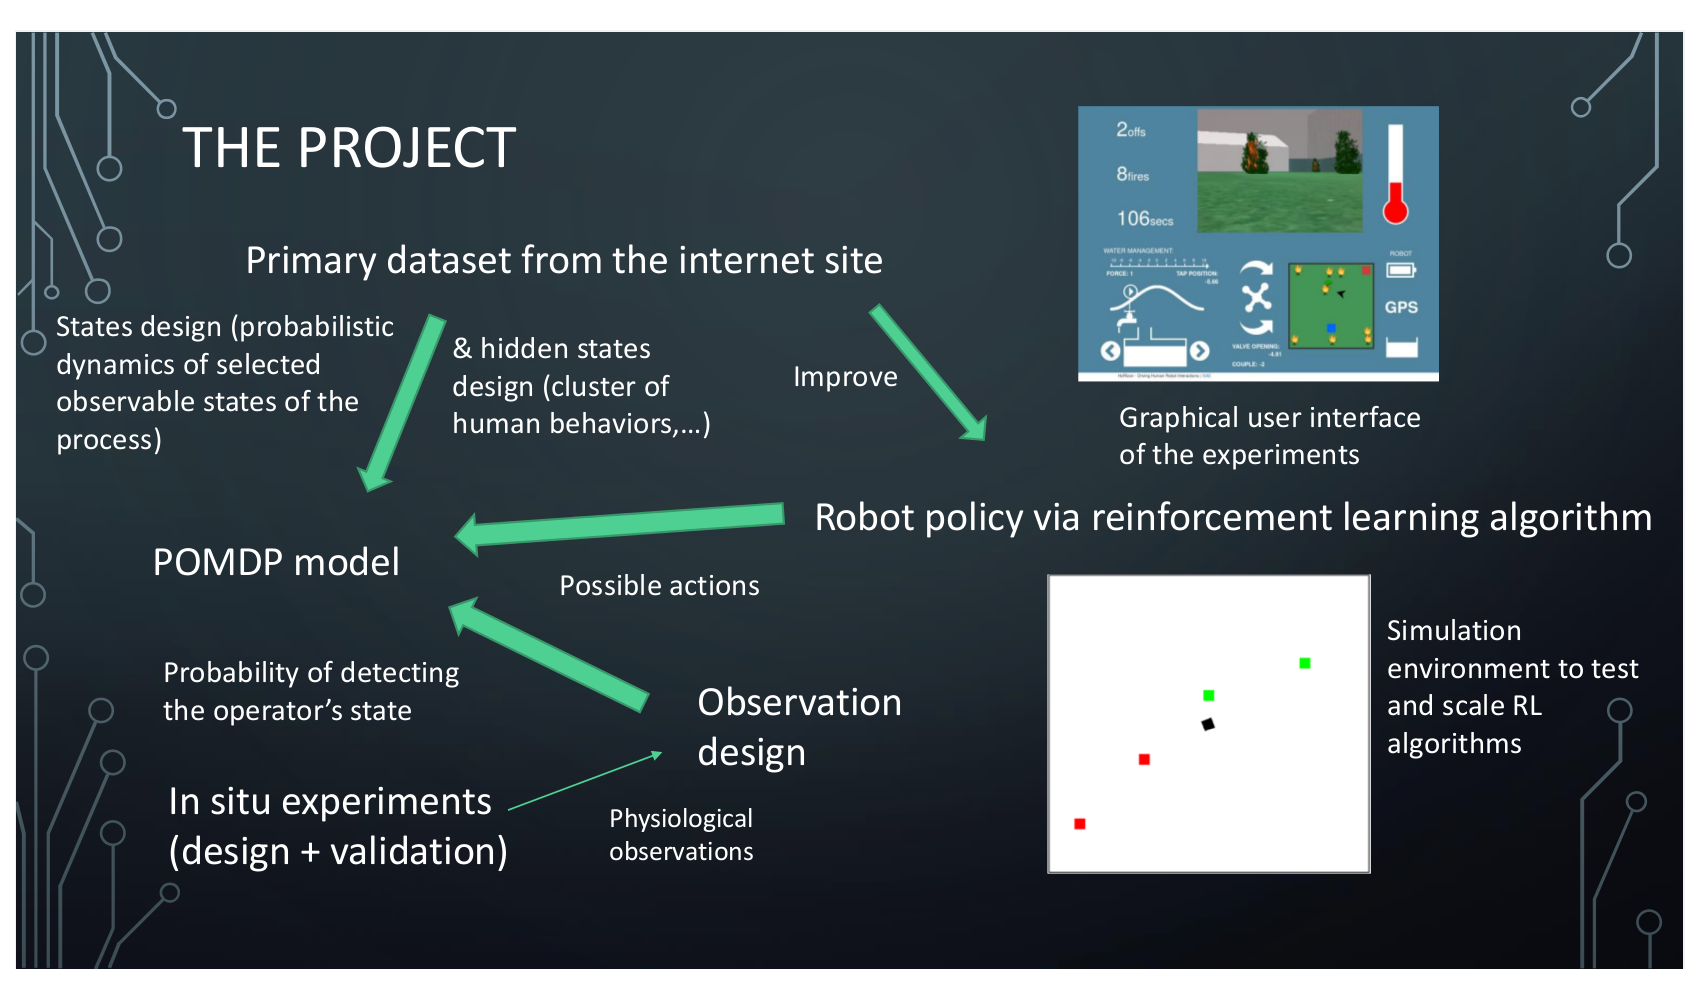
\includegraphics[scale = 0.19]{Schema.png}
  \label{fig:my-figure}
\end{figure}
\end{frame}

%\begin{frame}
%\frametitle{\insertsection}
%\framesubtitle{\footnotesize User Interface}
%\begin{figure}
%  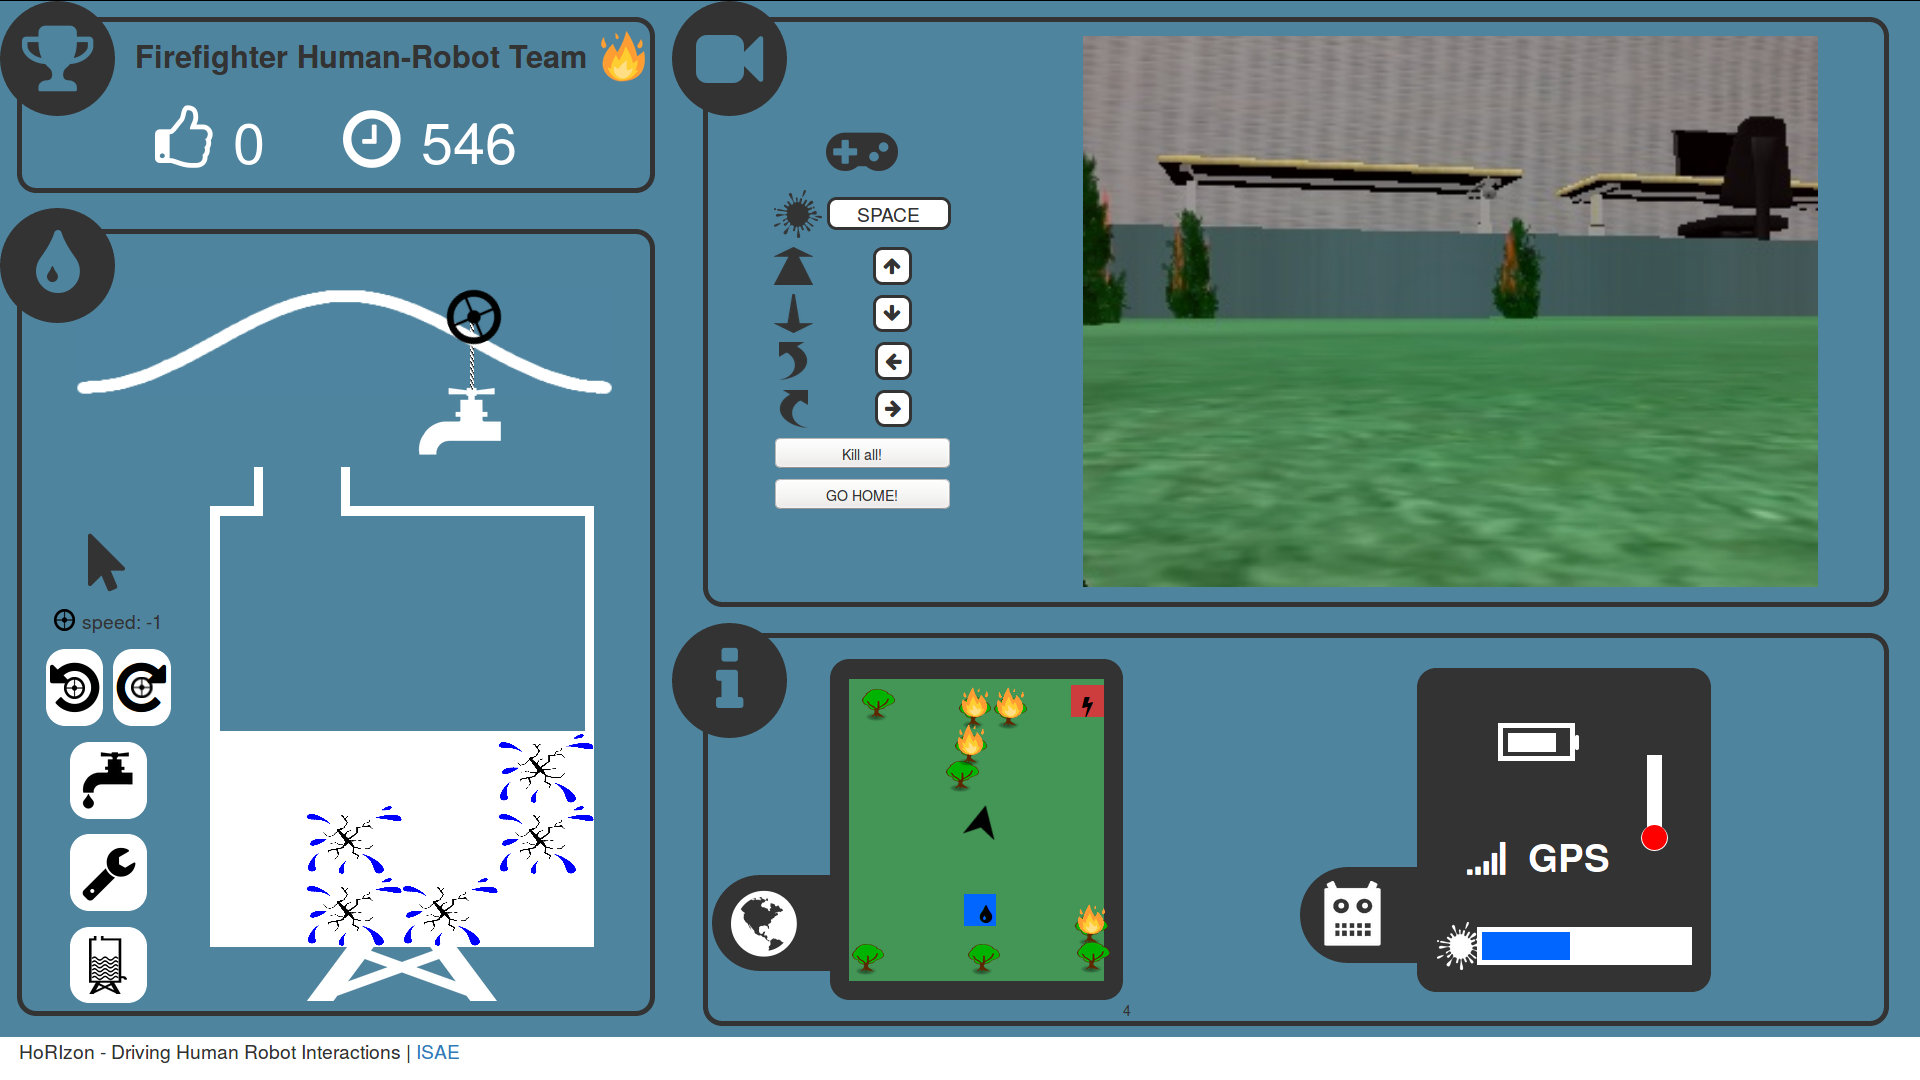
\includegraphics[scale = 0.15]{Website.png}
%  \label{fig:my-figure}
%\end{figure}
%\end{frame}

\section[theory]{Theory}

\begin{frame}
\frametitle{\insertsection}
\framesubtitle{\footnotesize History}
\textbf{Domain's birth} : late 70's by the encounter of
\begin{itemize}
\item experimental psychology 
\item computational neuroscience
\item dynamic programming
\end{itemize}
\visible<2->{
\begin{block}{\small{An approach to experimental psychology : Law of effects (Thorndike, 1911)}}
" The greater the satisfaction or discomfort, the greater the strengthening or weakening of the bond".
\end{block}
}
\end{frame}

\begin{frame}
\frametitle{\insertsection}
\framesubtitle{\footnotesize Reinforcement Learning}
\begin{block}{What is Reinforcement Learning?}
It is an approach, here computational, to decision-making, understanding and goal-directed learning. 
\end{block}
\visible<2->{
\textbf{What does it needs?}
The definition of the interactions between a learning agent and its environment.
\begin{itemize}
 \item the states
 \item the actions
 \item the rewards
\end{itemize}
}
\visible<3->{
\begin{block}{\textbf{RL objectives :}}
 the automatized acquisition of skills for decision making in a complex and uncertain environment and learning by "experience" a behavioral strategy (named policy) reflecting the failures and success (reinforcements or rewards).
\end{block}
}
\end{frame}

\begin{frame}
\frametitle{\insertsection}
\framesubtitle{\footnotesize Markov Property and Markov Chain}
\begin{block}{Markov property}
all the useful information for the future prediction is in the present state. 
\end{block}
\visible<2->{
\begin{block}{\textbf{Markov Chain}}
a dynamic system with discrete time $(x_t)_{t\in\mathbb{N}} \in X$, where $X$ is space of states such as :

\begin{equation*}
\mathbb{P}(x_{t+1}=x|x_t,x_{t-1},...,x_0)=\mathbb{P}(x_{t+1}=x|x_t).
\end{equation*}
\end{block}
}
\end{frame}


\begin{frame}
\frametitle{\insertsection}
\framesubtitle{\footnotesize Markov Decision Process}
\begin{block}{\textbf{Markov Decision Process (MDP)}}
defined by $(X,A,p,r)$, where :
\begin{itemize}
 \item $X$ space of states
 \item $A$ space of actions
 \item $p(y|x,a)$ : probability of transition from a state $x \in X$ to $y \in X$ when the action $a \in A$ is chosen:
 \begin{equation*}
 p(y|x,a) = \mathbb{P}(x_{t+1}=y|x_t=x,a_t=a),
 \end{equation*}
 \item $r(x,a,y)$ : reward when passing from $x$ to $y$ using the action $a$.
\end{itemize}
\end{block}
\end{frame}

\begin{frame}
\frametitle{\insertsection}
\framesubtitle{\footnotesize Value function and Bellman operator}
\begin{block}{\textbf{Value function}}
The value function are defined over the state space : \\
for $x \in X, V(x)$ is the mean of the sum of the rewards over time for a process starting in $x$.
\[ V^{\pi}(x) = \mathbb{E} [ \sum_{t \geqslant 0} r(x_t,\pi(x_t))  ] \]
\end{block}
\visible<2->{
\begin{block}{\textbf{Bellman operator}}
Written $T^{\pi}$, it is defined by : \\
\[ T^{\pi}=V^{\pi}(x) = r(x,\pi(x)) + \sum_{x'} p(x'|x,a)V(x') \]
\end{block}
}
\end{frame}


\begin{frame}
\frametitle{\insertsection}
\framesubtitle{\footnotesize Some solving methods}
\begin{itemize}
 \item \textbf{Direct solving} of the linear system $(I-\gamma P^{\pi})V^{\pi} = r^{\pi}$. That's the Gauss elimination method, but it have a complexity of $O(N^3)$
 \visible<2->{
 \item \textbf{Iteration on the values for a permanent policy} : we iterate on the operator $T^{\pi}$ (Bellman operator). Considering a given value function $V_0$, $V_{n+1} = T^{\pi} V_n$. 
We have then convergence of $V_n$ toward $V^{\pi}$. The problem is that the convergence is asymptotical, but the advantage is that it as a lower complexity than the direct solving method ($O(N^2 \frac{log(1/\epsilon)}{log(1/\gamma)})$ for an approximation of $\epsilon$ (interesting if $\gamma$ is not too close from 1)).
}
\end{itemize}
\end{frame}

\begin{frame}
\begin{itemize}
 \item \textbf{Monte-Carlo} : we simulate n trajectories $((x_t^i)_{t \geqslant 0})_{1 \leqslant i \leqslant n}$, starting from $x$ and following the policy $\pi$ : $x_{t+1}^i ~ p(.|x_t^i,\pi(x^i_t))$ , so :
 \begin{equation*}
 V^{\pi}(x) \approx \frac{1}{n} \sum_{i=1}^n \sum_{t \geqslant 0} \gamma^t r(x^i_t, \pi(x^i_t)).
 \end{equation*}
 this method is interesting if we want to evaluate a unique state. It has an approximation error of order $O(1/\sqrt{n})$
 \visible<2->{
 \item \textbf{Temporal differences TD($\lambda$)} : This is a smart method for using the trajectories to evaluate all the states crossed by those trajectories, by evaluating the value of a state $x$, by the sum of the observed temporal differences $r_t+\gamma V(x_{t+1}) - V(x_t)$ at the future instants t, weighted by a "trace" $\lambda$.
 }
\end{itemize}
\end{frame}

\begin{frame}
The impact of the temporal differences of future transitions on the estimation of the current state value is controled by $\lambda$. TD($\lambda$) is a compromise between : 
\begin{itemize}
 \item \textbf{TD($0$)} (to estimate the fixed point of the operator of Bellman $T^{\pi}$): 
 \begin{equation*}
  V_{n+1}(x_k) = V_n(x_k) + \eta_n(x_k)d_k. 
 \end{equation*}
 \item \textbf{TD(1)} (to estimate the mean): 
 \begin{equation*} 
 V_{n+1}(x_k) = V_n(x_k) + \eta_n(x_k)\sum_{l\geqslant k}d_l. 
 \end{equation*} 
\end{itemize}
\visible<2->{
\textbf{the choice of $\lambda$} :
\begin{itemize}
 \item $\lambda < 1$ allows to reduce the variance of the estimators compared with $\lambda=1$.
 \item $\lambda > 0$ allows to propagate faster the rewards compared with $\lambda=0$.
\end{itemize}
}
\end{frame}

\begin{frame}
\frametitle{\insertsection}
\framesubtitle{\footnotesize TD($\lambda$)}
\textbf{the algorithm TD($\lambda$)} %\cite{sutton1988learning}:
 After the observation of a trajectory $(x_0,x_1,...,x_K = 0)$, we update $V_n$	 to the states $(x_k)_0 \leqslant k<K$ following :
\begin{eqnarray*}
V_{n+1}(x_k) = V_n(x_k) + \eta_n(x_k)\sum_{l=k}^{K-1}\lambda^{l-k}d_l,\\ 
\mbox{ where } d_l = r^{\pi}(x_l) + V_n(x_{l+1})-V_n(x_l).
\end{eqnarray*}
with $\eta_n$ the learning step, typically $\frac{1}{n}$.

\end{frame}



\begin{frame}
\textbf{the algorithm TD($\lambda$)} in the actuated case :
We can define the actuated value function when, at each time step,
the process is stopped with probability $1 - \gamma$ with $0 < \gamma <1$:
\[ V^{\pi}(x) = \mathbb{E} [ \sum_{t \geqslant 0} \gamma^t r(x_t,\pi(x_t))  ]. \]
Algorithm TD($\lambda$) becomes
\begin{equation*}
V_{n+1}(x_k)=V_n(x_k)+\eta_n(x_k)\sum_{t \geqslant k}(\gamma \lambda)^{l-k}d_l.
\end{equation*}
\end{frame}

\section[experiment]{Experiment}

\begin{frame}
\frametitle{\insertsection}
\framesubtitle{\footnotesize The mission}
A search and fight type mission : the firefighter\\

\visible<2->{
\textbf{The objectives} : extinguish the maximum number of fire\\
} \visible<3->{
\textbf{The drawbacks :}
\begin{itemize}
 \item the battery
 \item the water level
 \item the temperature
\end{itemize}
}
\visible<3->{
\begin{figure}
  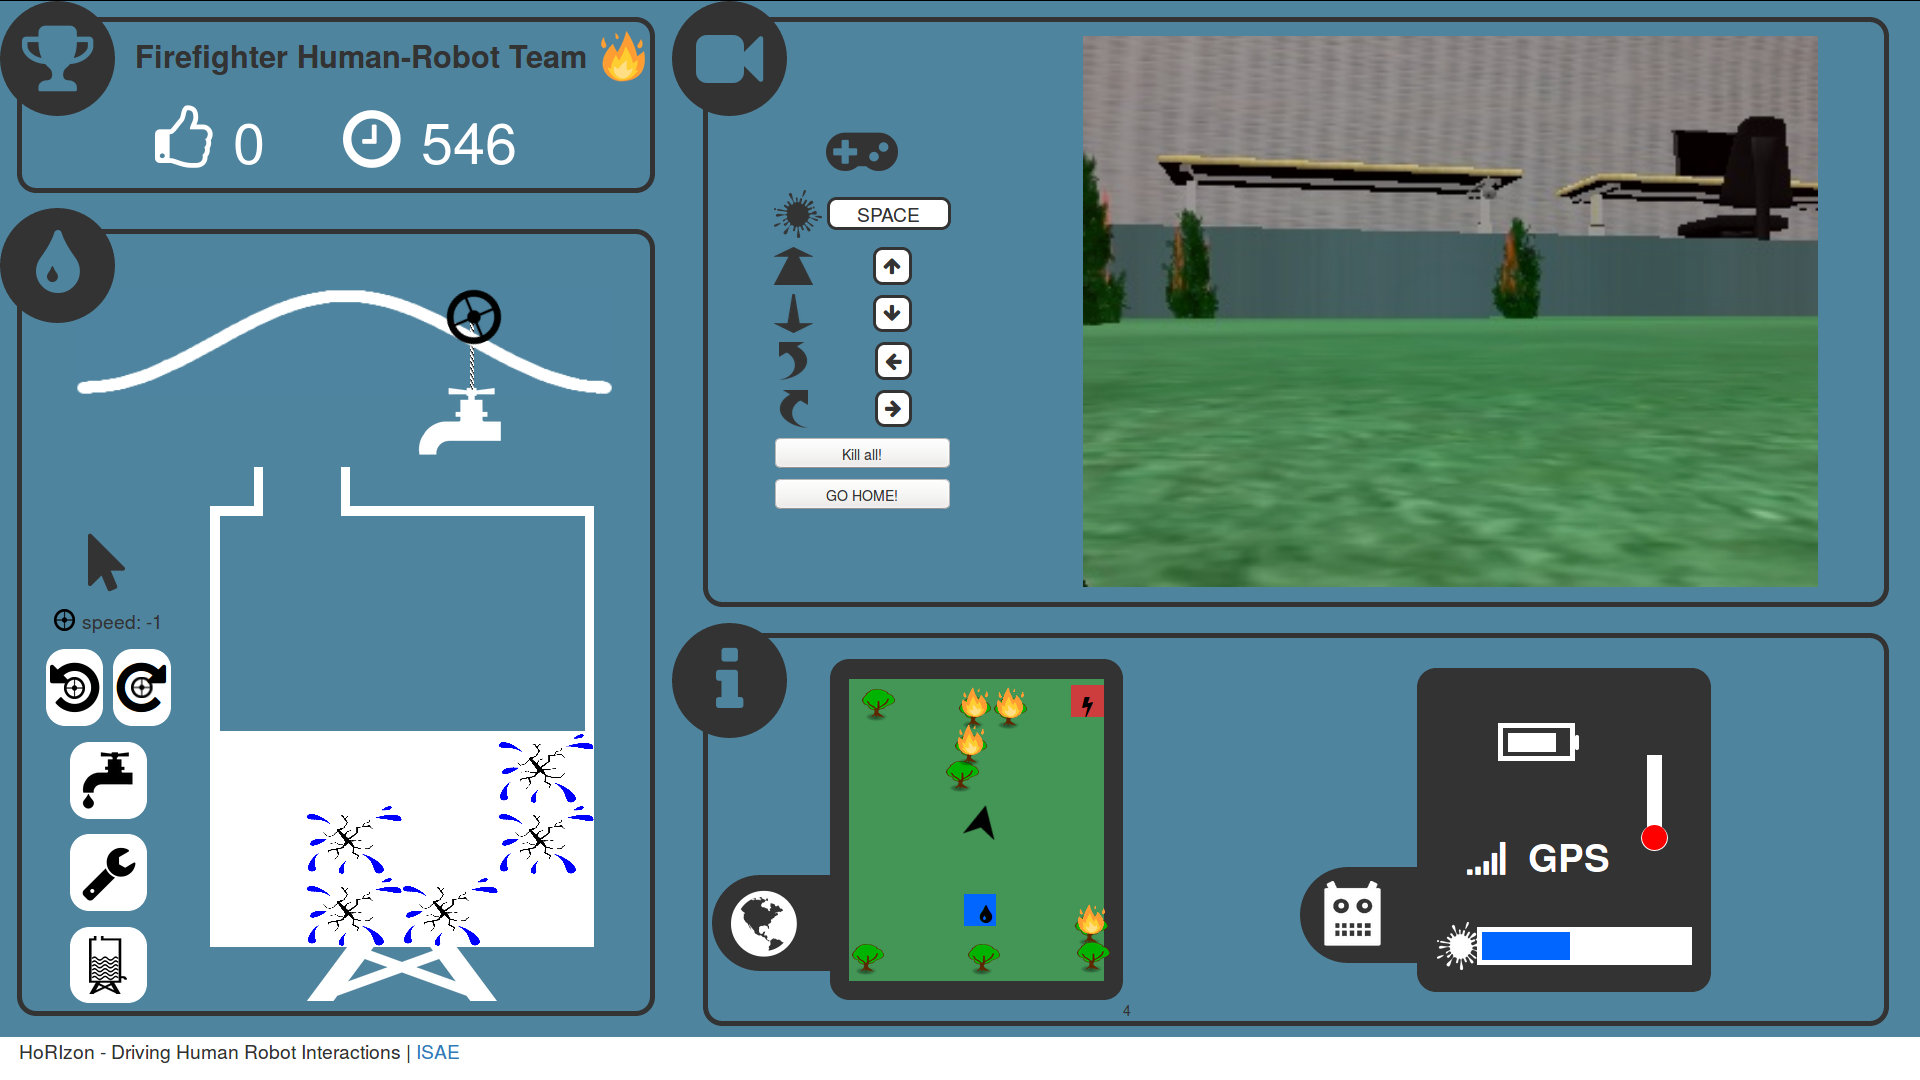
\includegraphics[scale = 0.13]{Website.png}
  \label{fig:my-figure}
\end{figure}
}
\end{frame}



\begin{frame}
\frametitle{\insertsection}
\framesubtitle{\footnotesize The environments}
\begin{figure}
  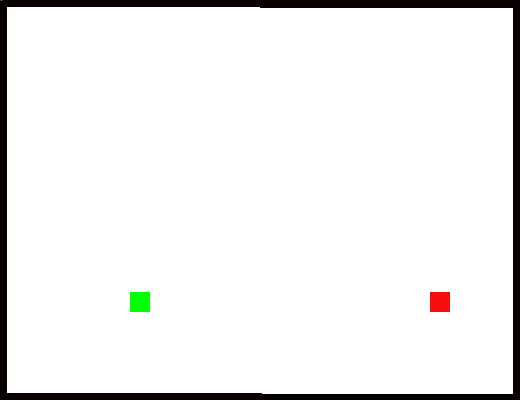
\includegraphics[scale = 0.2]{images/1Dultrasimple.png}
  \caption{View of the simulation of the simple environment}
  \label{fig:my-figure}
\end{figure}
\visible<2->{
\begin{figure}
  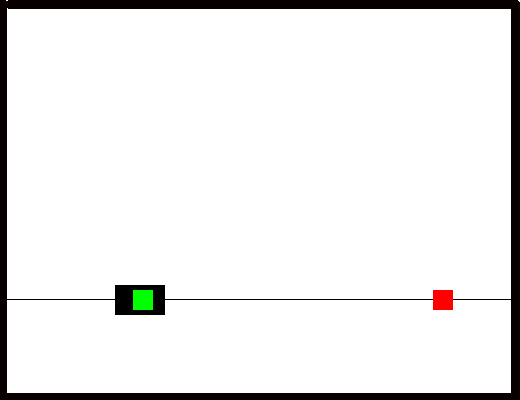
\includegraphics[scale = 0.2]{images/1Dsimple.png}
  \caption{View of the simulation of the 1D environment}
  \label{fig:my-figure}
\end{figure}
}
\end{frame}
\begin{frame}
\begin{figure}
  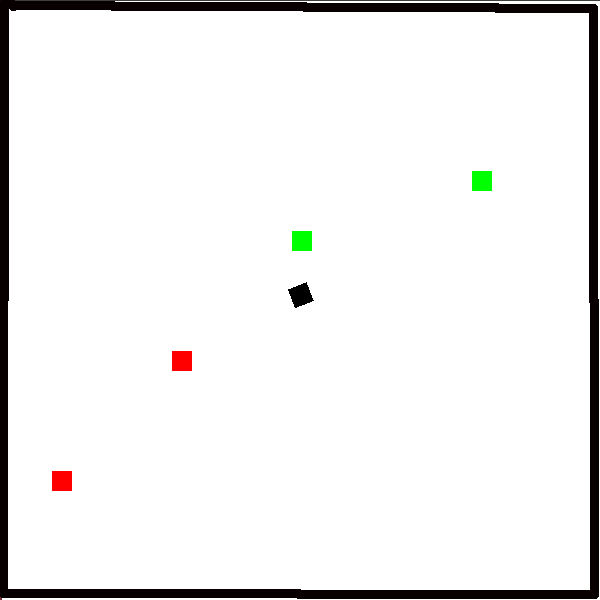
\includegraphics[scale = 0.3]{images/2Dsimple.png}
  \caption{View of the simulation of the 2D environment}
  \label{fig:my-figure}
\end{figure}
\end{frame}
\begin{frame}
\begin{figure}
  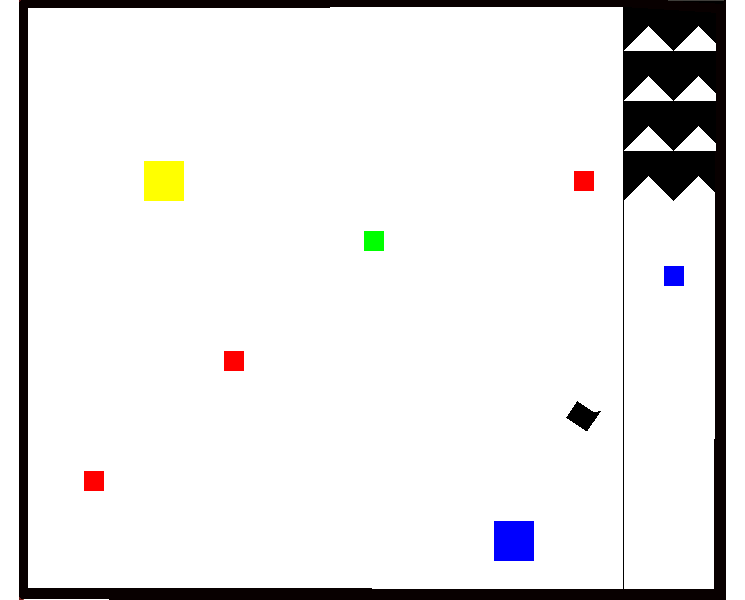
\includegraphics[scale = 0.3]{images/2Dcomplex.png}
  \caption{View of the simulation of the complex 2D environment}
  \label{fig:my-figure}
\end{figure}
\end{frame}

\begin{frame}
\frametitle{\insertsection}
\framesubtitle{\footnotesize Results}
\begin{figure}
\definecolor{ggreen}{rgb}{0.3,0.7,0.4}
\begin{tikzpicture}[scale = 0.6]
\begin{axis}[
grid=major,xmin=1,xmax=1000,ymin=-1,ymax=10,
xtick={0,100,...,1000},
legend entries={$\lambda = 0.02$,$\lambda = 0.1$,$\lambda = 0.01$,$\lambda = 0.5$,$\lambda = 0.005$,$\lambda = 0.8$,legend style={at={(1.52,1.1)}}},
xlabel={Number of episodes},
ylabel={Score},
title={Score growing during learning},width=11cm,height=11cm]
\addplot[color = black, line width=1pt] plot table[x index=0, y index=1]{CSV/origin.csv};
\addplot+[color = blue, line width=1pt] plot table[x index=0, y index=1]{CSV/ralpha_01.csv};
\addplot+[color = red, line width=1pt] plot table[x index=0, y index=1]{CSV/ralpha_001.csv};
\addplot+[color = orange, line width=1pt] plot table[x index=0, y index=1]{CSV/ralpha_05.csv};
\addplot+[color = purple, line width=1pt] plot table[x index=0, y index=1]{CSV/ralpha_0005.csv};
\addplot+[color = brown, line width=1pt] plot table[x index=0, y index=1]{CSV/ralpha_08.csv};

\end{axis}
\end{tikzpicture}
\caption{Score of the deterministic 1D environment for $\lambda$}
\end{figure}

\end{frame}

\begin{frame}
\begin{figure}
\definecolor{ggreen}{rgb}{0.3,0.7,0.4}
\begin{tikzpicture}[scale = 0.6]
\begin{axis}[
grid=major,xmin=1,xmax=1000,ymin=-1,ymax=10,
xtick={0,100,...,1000},
legend entries={$\gamma = 1$,$\gamma = 0.5$,$\gamma = 0.7$,$\gamma = 0.3$,legend style={at={(1.52,1.1)}}},
xlabel={Number of episodes},
ylabel={Score},
title={Score growing during learning},width=11cm,height=11cm]
\addplot[color = black, line width=1pt] plot table[x index=0, y index=1]{CSV/gamma1.csv};
\addplot+[color = blue, line width=1pt] plot table[x index=0, y index=1]{CSV/gamma05.csv};
\addplot+[color = red, line width=1pt] plot table[x index=0, y index=1]{CSV/gamma07.csv};
\addplot+[color = orange, line width=1pt] plot table[x index=0, y index=1]{CSV/gamma03.csv};;

\end{axis}
\end{tikzpicture}
\caption{Score of the deterministic 1D environment for $\gamma$}
\end{figure}

\end{frame}

\begin{frame}
\begin{figure}
\definecolor{ggreen}{rgb}{0.3,0.7,0.4}
\begin{tikzpicture}[scale = 0.6]
\begin{axis}[
grid=major,xmin=1,xmax=1000,ymin=-1,ymax=10,
xtick={0,100,...,1000},
legend entries={$\epsilon = 0.2$,$\epsilon = 0.4$,$\epsilon = 0.1$,legend style={at={(1.52,1.1)}}},
xlabel={Number of episodes},
ylabel={Score},
title={Score growing during learning},width=11cm,height=11cm]
\addplot[color = black, line width=1pt] plot table[x index=0, y index=1]{CSV/origin.csv};
\addplot+[color = blue, line width=1pt] plot table[x index=0, y index=1]{CSV/epsilon4.csv};
\addplot+[color = red, line width=1pt] plot table[x index=0, y index=1]{CSV/epsilon1.csv};

\end{axis}
\end{tikzpicture}
\caption{Score of the deterministic 1D environment for $\epsilon$}
\end{figure}
\end{frame}

\section[conclusion]{Conclusion}

\begin{frame}
\center
{\huge Conclusion}
\end{frame}

\begin{frame}
        \frametitle{\hspace{0.3cm} 
\includegraphics[scale=0.35,trim= 0 0 0 -0.3cm]{logo2015} }
	\vspace{-0.2cm}
	\bibliographystyle{alpha}	
	{\tiny        
		\bibliography{main}
	}
	\vspace{0.2cm}
	\hspace{5cm} {\huge \textbf{Thank you!} }
\end{frame}



%}
\end{document}
